\chapter{Fundamentals}
\label{fundamentals}

This chapter starts with a short overview of the SimTech project, of which this diploma thesis is a part of.
Next, bootstrapping is defined in the context of this diploma thesis, since it can have various different meanings.
Then, a short overview of the cloud landscape is presented, with focus on Amazons cloud offerings, since these are used in this diploma thesis.
Finally, we take a look at provisioning solutions, in particular TOSCA, which is also used later in this thesis.

\section{SimTech}
\label{fundamentals:simtech}

Since 2005, the German federal and state government have been running the Excellence Initiative\footnote{\url{http://www.dfg.de/en/research_funding/programmes/excellence_initiative/index.html}}, which aims to promote cutting-edge research, thereby increasing the quality and international competitiveness of German universities.
In three rounds of funding, universities have competed with project proposals in three areas: Institutional Strategies, Graduate Schools, and Clusters of Excellence.
\nom{Simulation Technology}{SimTech} is one of the Clusters of Excellence that are funded by the Excellence Initiative.
In a partnership between the University of Stuttgart, the German Aerospace Center, the Fraunhofer Institute for Manufacturing Engineering and Automation, and the Max Planck Institute for Intelligent Systems, it combines over 60 project from researchers in Engineering, Natural Science, and the Life and Social Sciences.
The aim of SimTech is to improve existing simulation strategies and to create new simulation solutions~\autocite{excellence:glance}.

In the SimTech project, seven individual research areas collaborate in seven different project networks, one of which is project network 6: \textit{Cyber Infrastructure and Beyond}.
The goal of this project network is to build an easy-to-use infrastructure that supports scientists in their day to day work with simulations~\autocite{simtech:projectnetwork6}.

\subsection{SimTech SWfMS}

As part of this project, the SimTech SWfMS was developed.
It is a system that enables scientists to easily create, manage and execute simulation workflows which are a subcategory of scientific workflows~\autocite{workflow:simulation:flexibility}.
The SimTech SWfMS introduces extensions to the BPEL language that add functionality to support the requirements of simulation workflows, such as passing data by reference to support larger amounts of data often found in science~\autocite[also~see][]{workflow:simulation:modelling:datareferences}, or shared context between workflows~\autocite{workflow:simulation:modelling}.
Other extension introduces by the SimTech SWfMS to support simulation workflows include a service bus that supports late binding, rebinding, and legacy simulation software, as well as the \nom{Simulation Data Management System}{SIMPL} that provides unified access methods for arbitrary external data~\autocite{workflow:simulation:runtime}.
Additionally, extension where also made in the areas of flexibility to support a "model as you go" approach and in human user involvement to support human tasks for decision making, data manipulation, or workflow repair~\autocites{workflow:simulation:flexibility}{workflow:simulation:humanusers}.

The SimTech SWfMS consists of the \nom{SimTech Workflow Modeling \& Monitoring Tool}{SimTech Modeler} and the workflow middleware.
The SimTech Modeler is based on Eclipse JEE\footnote{\url{http://www.eclipse.org/ide/}} and extends its functionality with various plugins.
\autoref{image:modeler} shows the SimTech Modeler user interface.
It allows the user to create simulation workflows using a graph as visual representation, where vertices represent simulation tasks and edges describe the progression between those tasks.

\begin{figure}[!htbp]
	\centering
	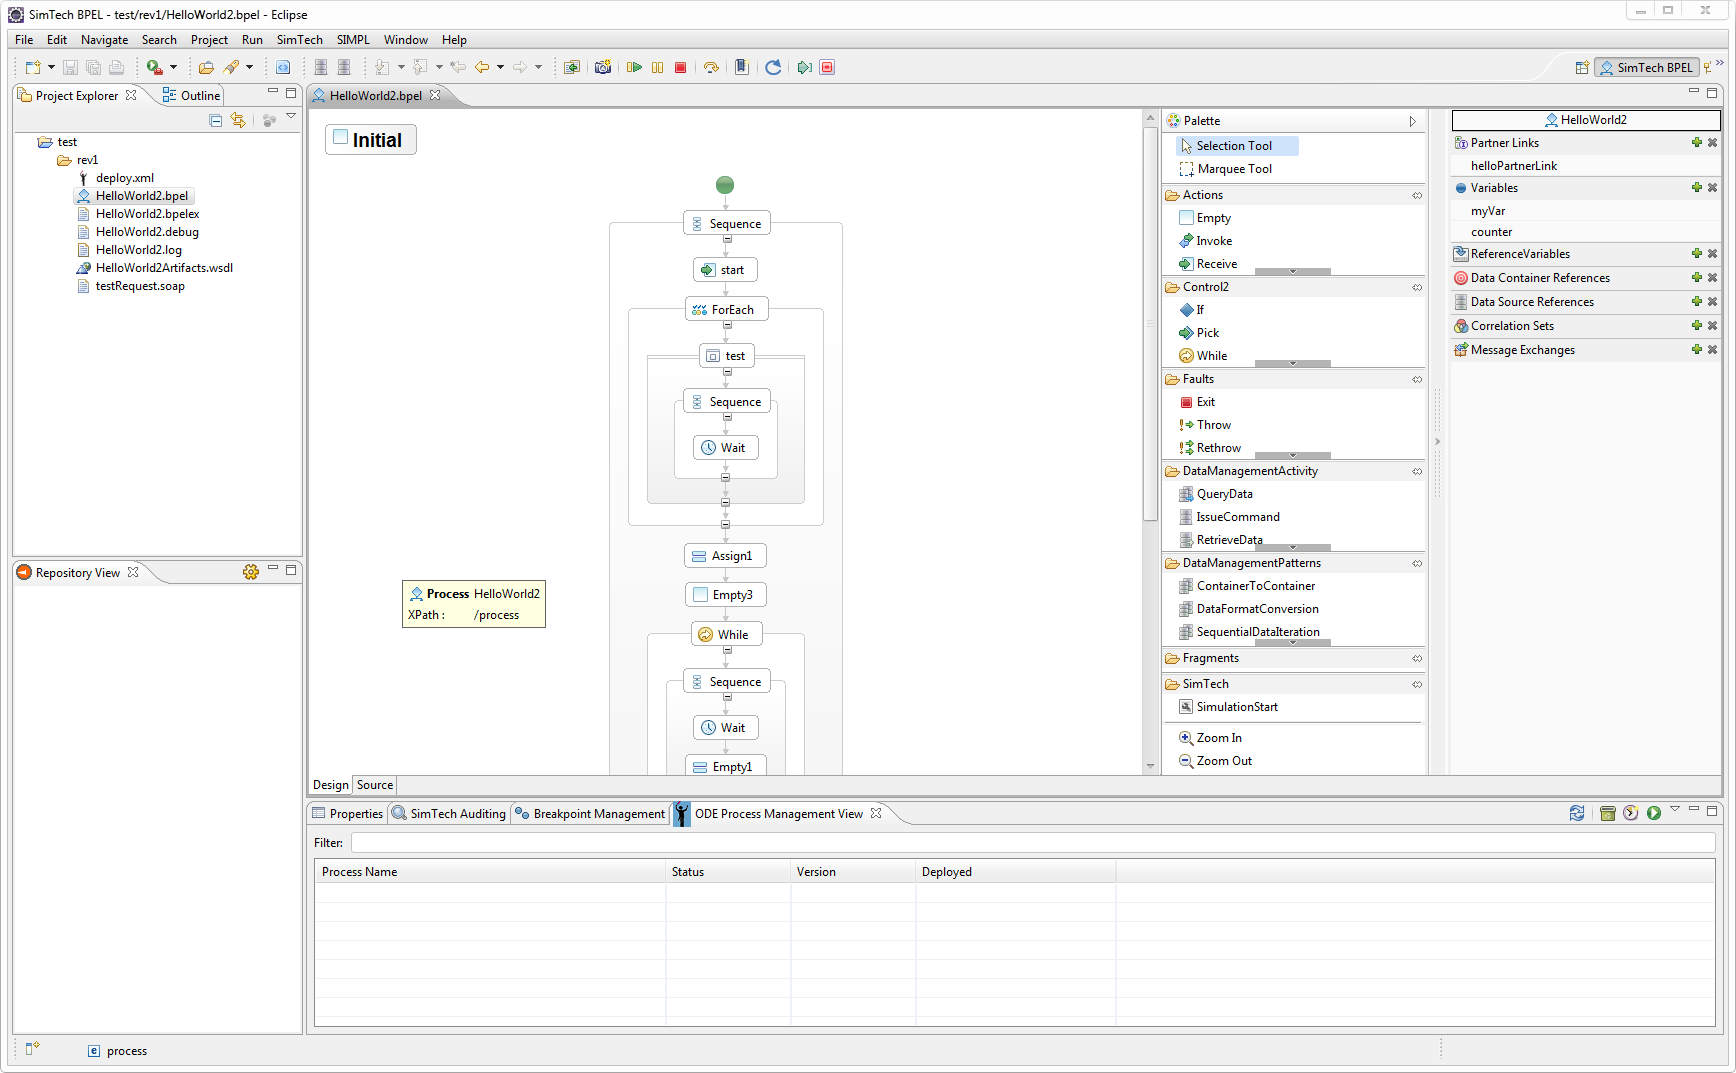
\includegraphics[width=\textwidth,interpolate=false]{fundamentals/assets/simtech_modeler}
	\caption{The SimTech Modeler user interface.}
	\label{image:modeler}
\end{figure}

Once the user is done modeling the simulation workflow, he clicks on a button to execute the workflow on the workflow middleware.
The middleware consists of various components that are executed by an application server, in this case Apache Tomcat\footnote{\url{http://tomcat.apache.org/}}.
The workflow is deployed on the workflow engine, in this case \nom{ODE Pluggable Framework}{ODE-PGF}\footnote{\url{http://www.iaas.uni-stuttgart.de/forschung/projects/ODE-PGF/}}, which executes the workflow step by step.
If a step involves the execution of a service, the ESB (Apache Service Mix) is called, who resolves the services and passes along the request and the response.

\section{Bootstrapping}
\label{fundamentals:bootstrapping}

The term \textit{to bootstrap sth.} appears to have originated in the early 19th century in the United States, where phrases like "pulling oneself up over a fence by the straps of one's boots" where used as a figure for an impossible task~\autocite{bootstrap:history}.
In the early 20th century the metaphor's sense shifted to suggest a possible task, where one improves one's situation by one's own efforts without help from others.
An example of this can be found in James Joyce's Ulysses from 1922, where he writes about "others who had forced their way to the top from the lowest rung by the aid of their bootstraps"~\autocite{bootstrap:ulysses}.
From there, the metaphor extended to the general meaning it has today which is the act of starting a self-sustaining process that proceeds without help from the outside.

An early reference to bootstrapping in the context of computing dates back to 1953, describing the bootstrapping technique as follows: "Pushing the load button then causes one full word to be loaded into a memory address [...], after which the program control is directed to that memory address and the computer starts automatically. [This] full word may, however, consist of two instructions of which one is a \textit{Copy} instruction which can pull another full word [...], so that one can rapidly build up a program loop which is capable of loading the actual operating program"~\autocite{bootstrap:early}.

\pagebreak

The term bootstrapping is also used with a similar meaning in a business context, where it refers to the process of starting and sustaining a company without outside funding\footnote{\url{http://venturebeat.com/2008/11/20/the-art-of-the-bootstrap/}}.
The company is started with money from the founders, which is used to develop a product that can be sold to customers.
Once the business reaches profitability it is self-sufficient and can use the profits it generates to organically grow further.

In this diploma thesis, bootstrapping describes the process of starting a simple program that, without further help, is able to start much more complex programs.
These complex programs might require additional middleware, databases, or other components.
During the bootstrapping process, all these dependencies will be set up automatically.

\section{Cloud}

\section{Provisioning Solutions}

This section describes some of the provisioning solution available today, in particular TOSCA and Open TOSCA, since those are used in the prototypical implementation later on.

\subsection{TOSCA}

\nom{Topology and Orchestration Specification for Cloud Applications}{TOSCA} is a standard that is currently being worked on by the \nom{Organization for the Advancement of Structured Information Standards}{OASIS}\footnote{\url{https://www.oasis-open.org/}}.
Its development is also supported by various industry partners, which include IBM, Cisco, SAP, HP and others.
It's aim is to provide a language that can describe service components and their relations in a cloud environment independent fashion~\autocite{tosca:spec}.

TOSCA defines an XML syntax, which describes services and their relations in a so called service templates.
\autoref{image:tosca:servicetemplate} shows that a service template can be made of up of four distinct parts: Topology templates, orchestration plans, reusable entities, and artifact templates.

\begin{figure}[!htbp]
	\centering
	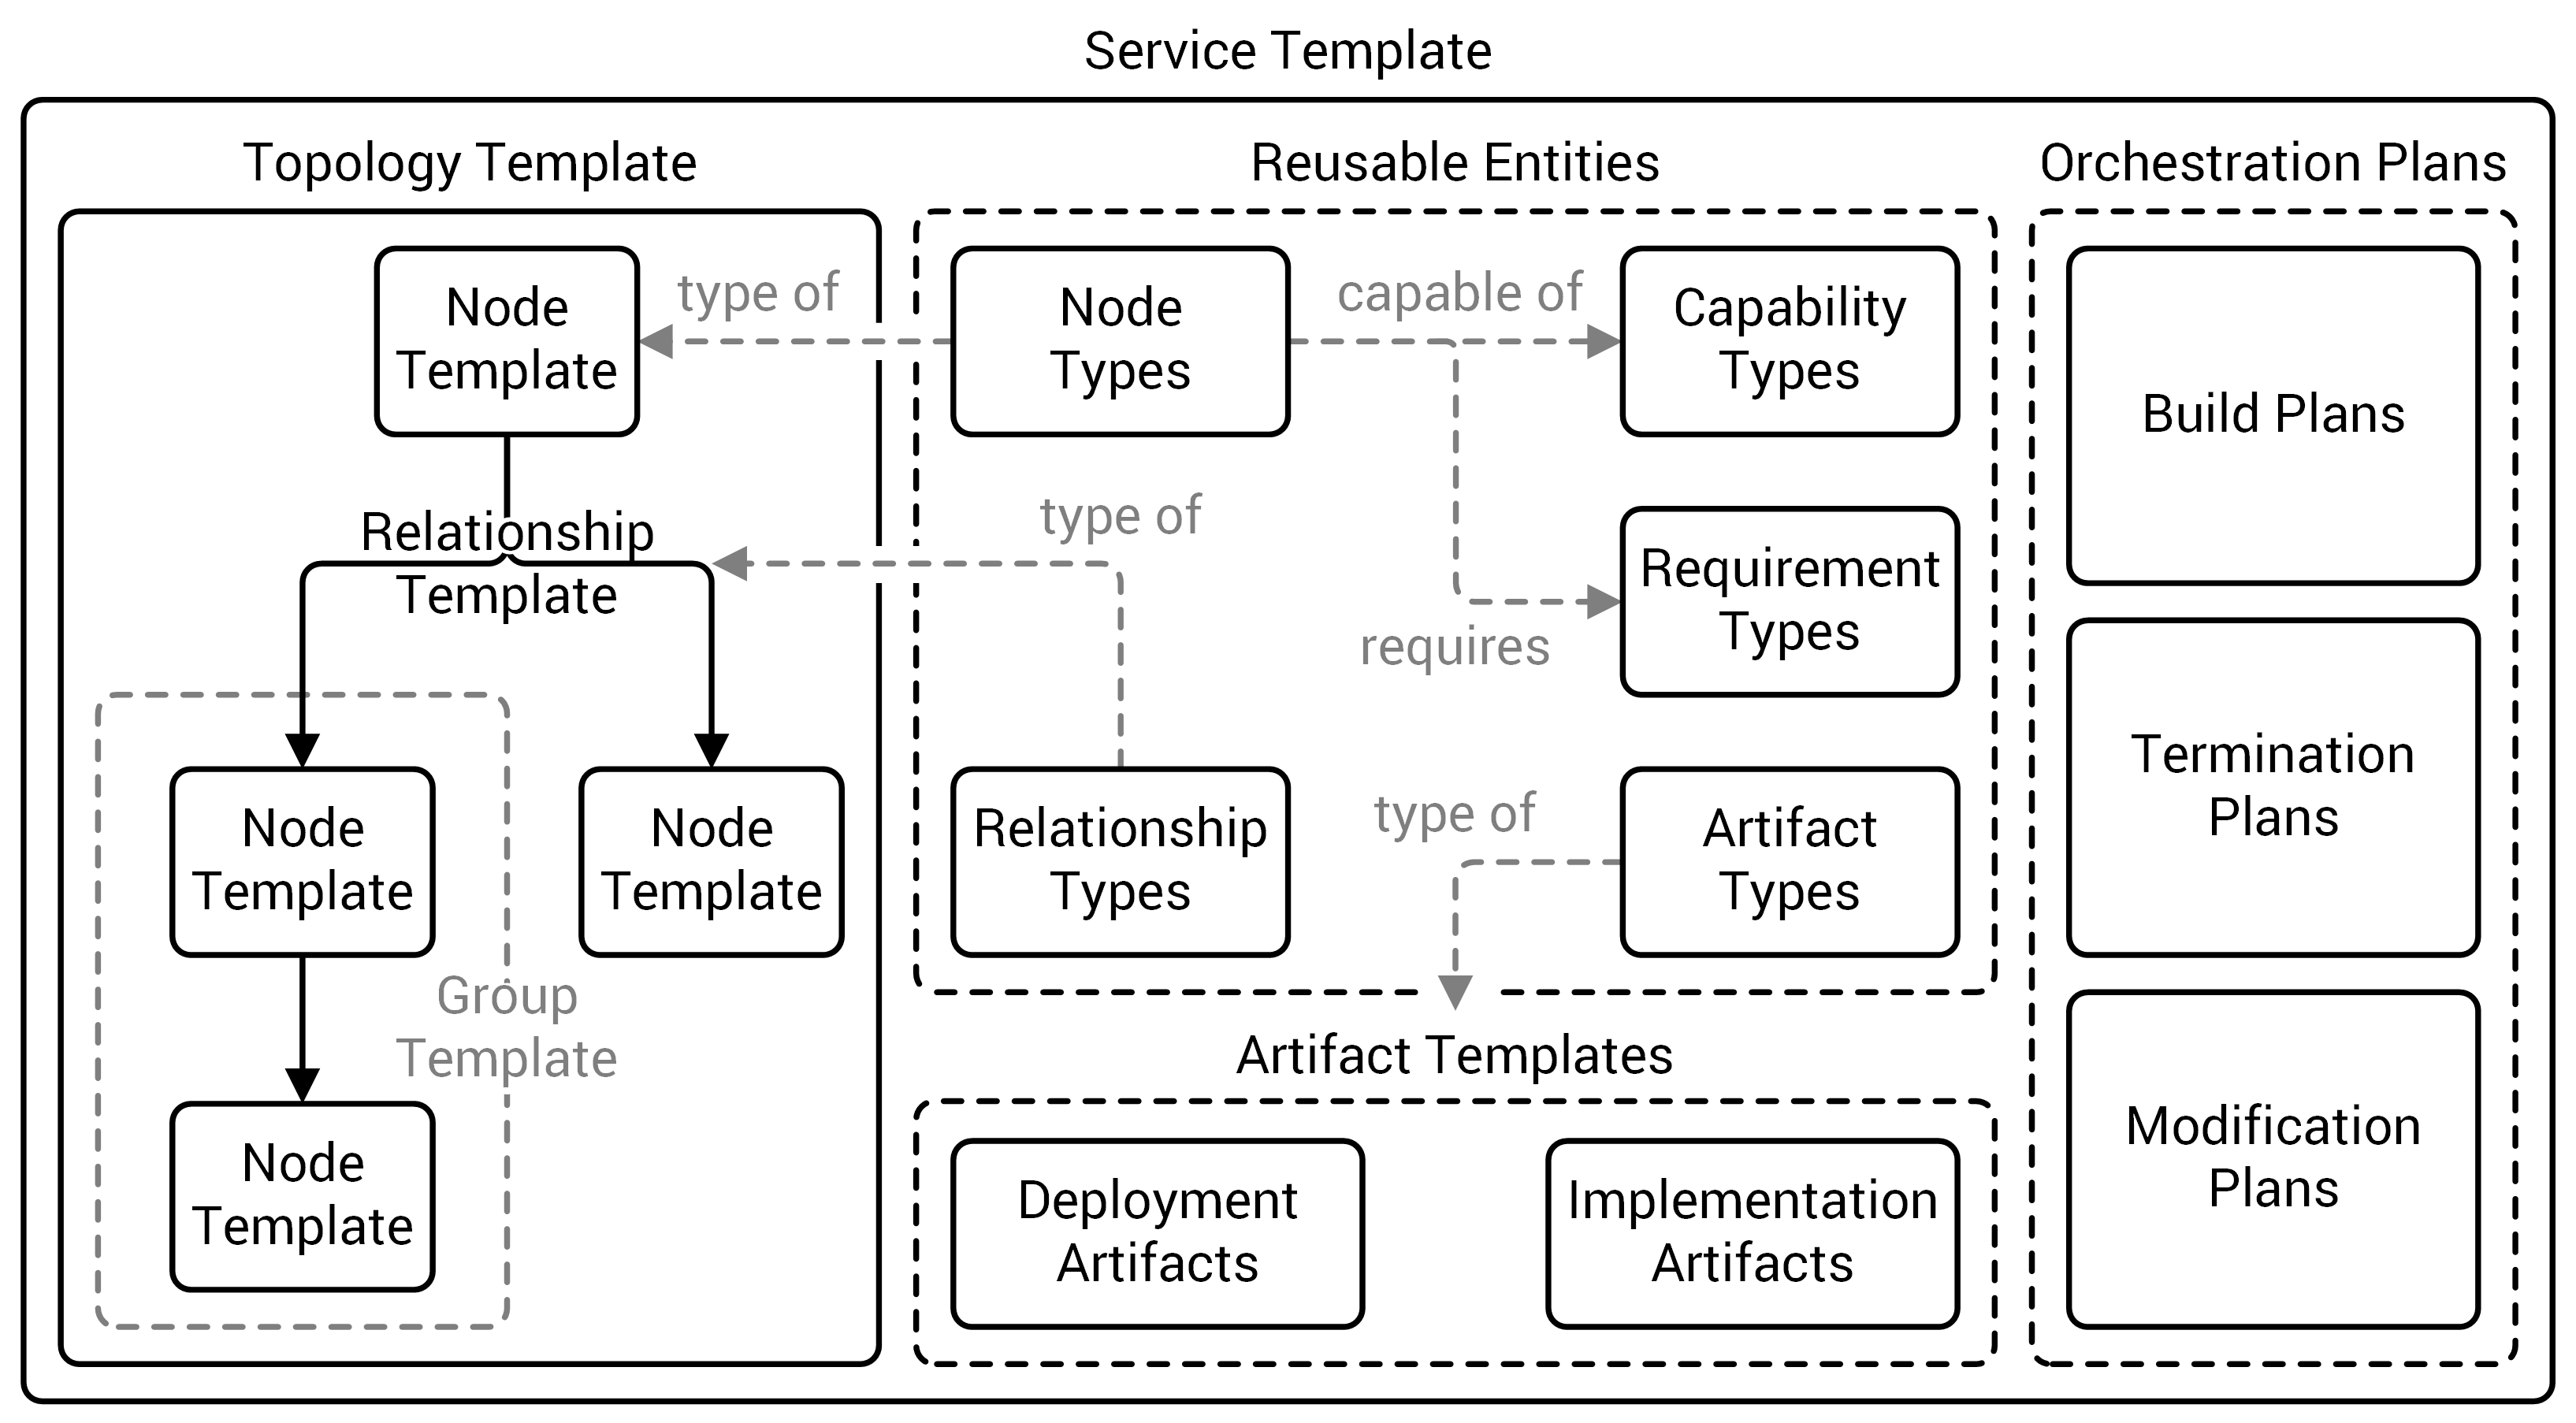
\includegraphics[resolution=600]{fundamentals/assets/service_template}
	\caption{TOSCA service template structure~\autocite[based on][]{tosca:spec}.}
	\label{image:tosca:servicetemplate}
\end{figure}

Topology templates, as seen on the left side of \autoref{image:tosca:servicetemplate}, model the structure of a service as a directed graph.
The vertices of the graph represent nodes, which are occurrences of a specific component, for example, an application server or a database.
These nodes are defined by node types, or by other service templates.
Node types are reusable entities,  as shown in the top center of \autoref{image:tosca:servicetemplate}.
They define the properties of a component, as well as operations to manipulate a component, so called interfaces.
Additionally, node types can be annotated with requirements and capabilities.
These, in turn, are defined by requirement and capability types, which also belong to the group of reusable entities.
This allows for requirement and capability matching between different components.
The edges of the graph represent connections between nodes, which are defined by relationship templates that specify the properties of the relation.
An example for such a connection would be a node A, representing a web service, which is deployed on node B, an application server.
Relationship types are also used to connect requirements and capabilities.

Orchestration plans, shown on the left of \autoref{image:tosca:servicetemplate}, are used to manage the service that is defined by the service template. TOSCA distinguishes between three types of plans: Build plans, termination plans, and modification plans.
Build plans describe, how instances of a service are created.
Termination plans describe, how such a service is removed.
Modification plans manage a service during its runtime.
These plans consist of one or more tasks, i.e., an operation on a node (via an interface) or an external service call, and the order in which these tasks should be performed.
They can be written in \nom{Business Process Model and Notation}{BPMN} or \nom{Business Process Execution Language}{BPEL}, which are already existing languages to describe process models.

The bottom center of \autoref{image:tosca:servicetemplate} shows artifact templates, which represent artifact.
Artifacts are things that can be executed directly (e.g.: scripts, archives) or indirectly (e.g.: URL, ports).
TOSCA further distinguishes between two types of artifacts, namely deployment and implementation artifacts.
Deployment artifacts materialize instances of a node and are used by a build plan to create a service.
An example for this is an \nom{Amazon Machine Images}{AMI}, which creates an Apache server once deployed in a VM.
Implementation artifacts represent the interfaces of components.
Here, an example would be a node that has an interface for starting the particular component described by the node.
This interfaces could be implemented by an implementation artifact like a \textit{.jar} file.

One or more TOSCA service templates are packaged, together with some meta data, into a \nom{Cloud Service Archive}{CSAR}, which is essentially a zip file that contains all files necessary to create and manage a service.bv
CSAR files can then be executed in a TOSCA runtime environment, also called TOSCA container, to create the service described within.

\subsection{OpenTOSCA}

OpenTOSCA is an browser based open-source implementation of a TOSCA container, created at the IAAS at University Stuttgart, which supports the execution of TOSCA CSAR archives.
\autoref{image:tosca:opentosca} shows the architecture of OpenTOSCA.
The functionality of OpenTOSCA is realized in three main components, which are the Controller, the Implementation Artifact Engine, and the Plan Engine.
After a CSAR is uploaded to OpenTOSCA it can be deployed in three steps.
In the first step, the CSAR file is unpacked and its content is stored for further use.
The TOSCA XML files are then loaded and processed by the Controller.
The Controller in turn calls the Implementation Artifact Engine and the Plan Engine.
The Implementation Artifact Engine knows how to deploy and store the provided implementation artifacts via plugins.
Plans are then run by the Plan Engine, which also uses plugins to support different plan formats.
OpenTOSCA also offers two APIs, the Container API and the Plan Portability API.
The Container API can be used to access the functionality provided by the container from outside and to provide additional interfaces to the container, like the already existing admin UI, self-service portal, or modeling tool.
The Plan Portability API is used by plans to access topology and instance information~\autocite{opentosca}.

\begin{figure}[!htbp]
	\centering
	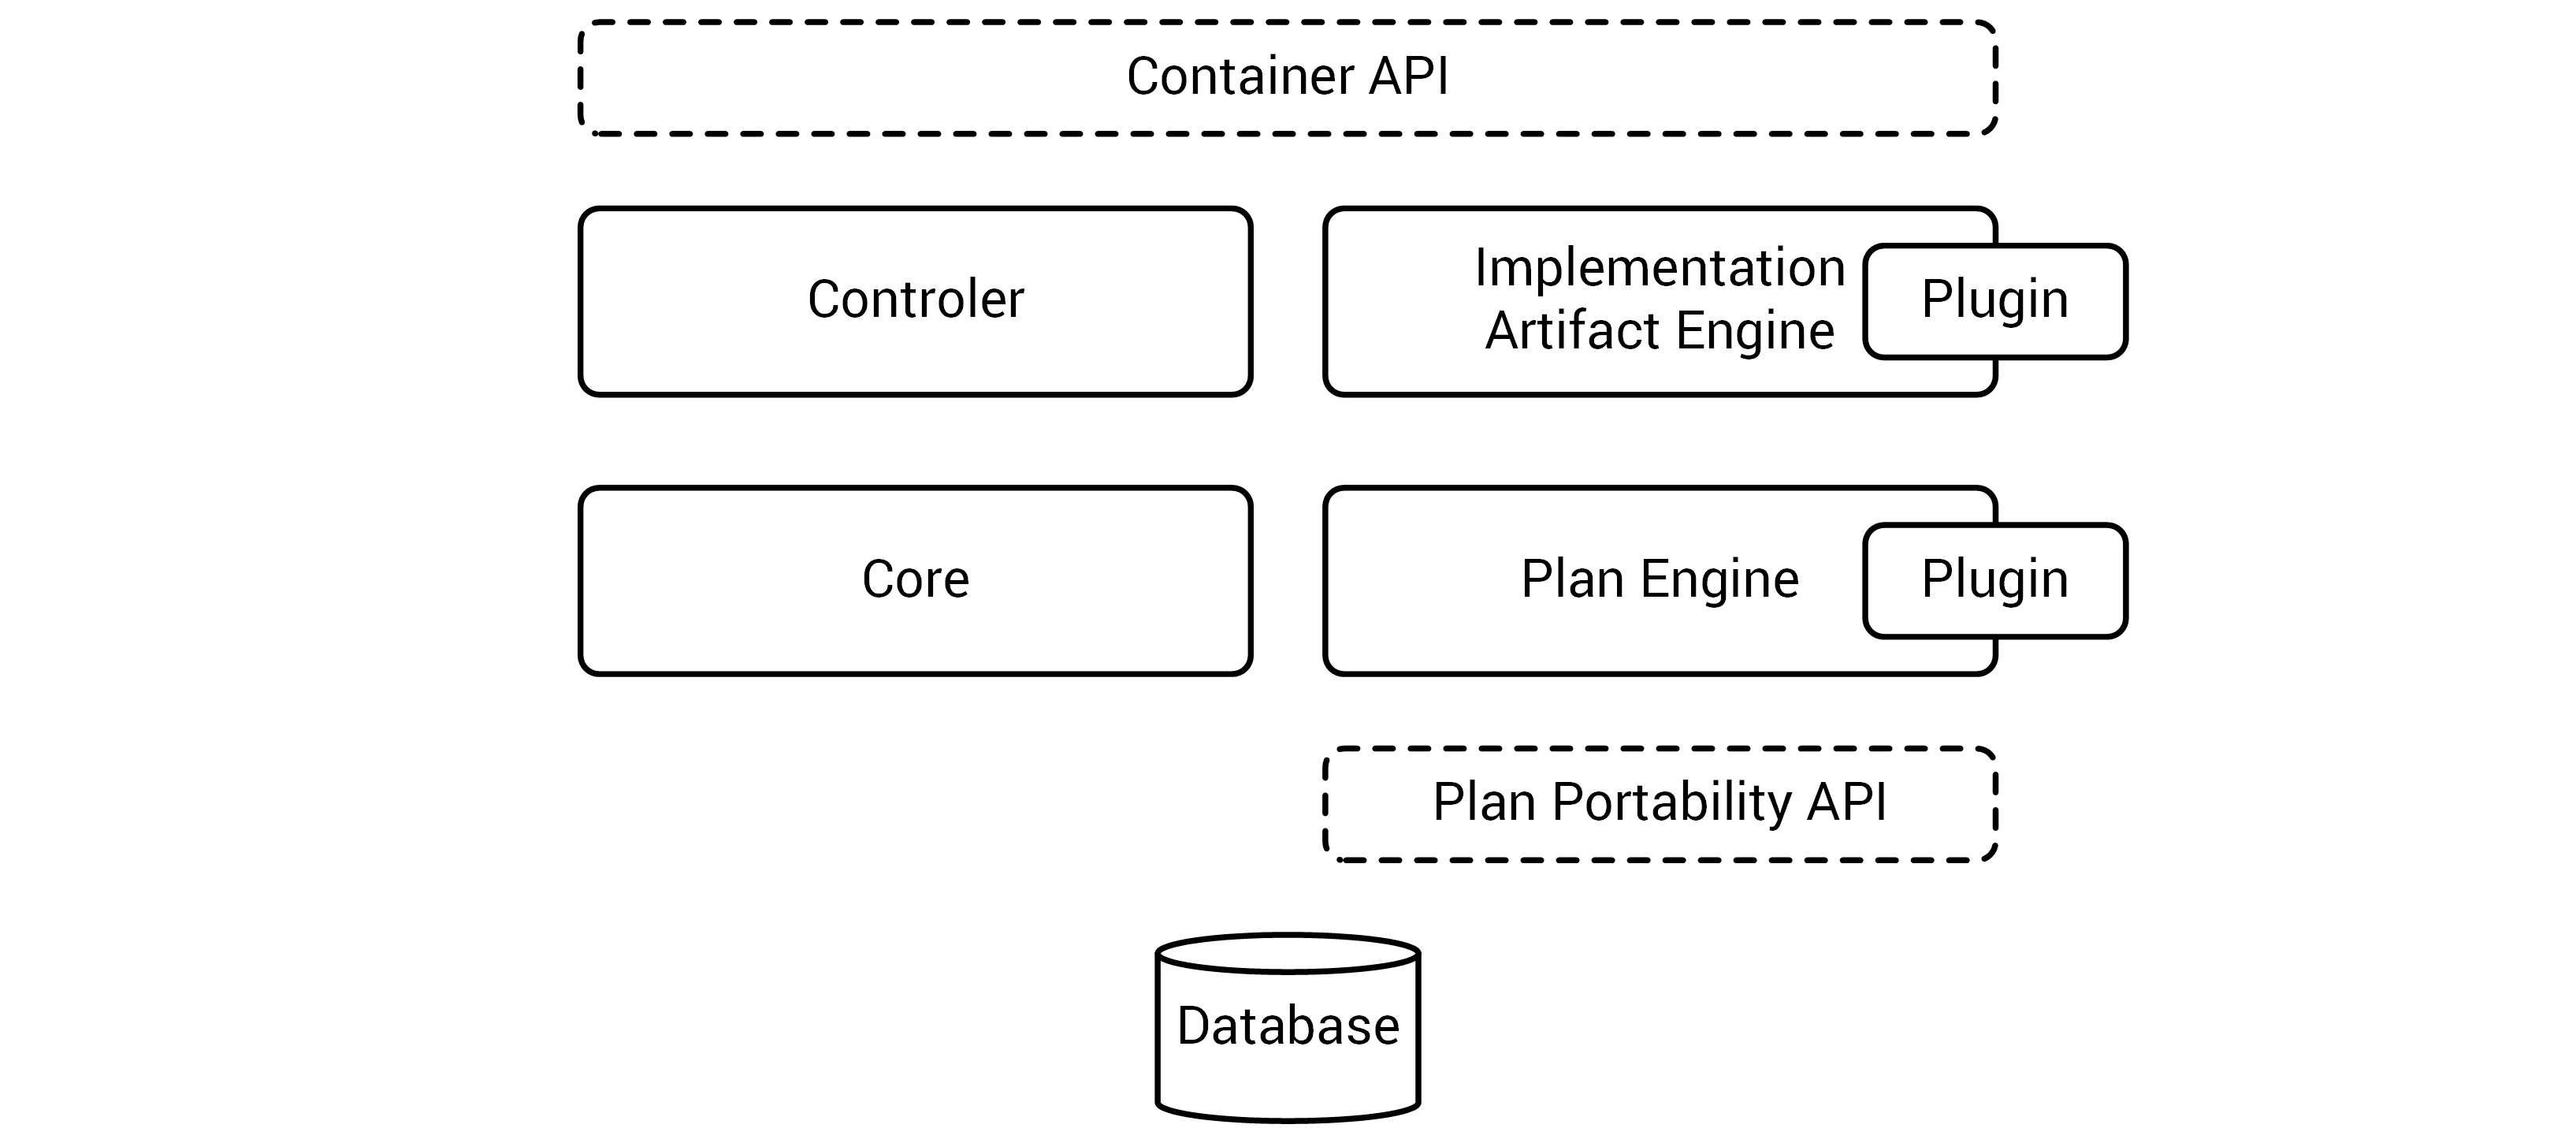
\includegraphics[resolution=600]{fundamentals/assets/opentosca}
	\caption{OpenTOSCA architecture~\autocite[based on][]{opentosca}.}
	\label{image:tosca:opentosca}
\end{figure}

